\documentclass[11pt]{article}
\usepackage{latexsym}
\usepackage{amsmath}
\usepackage{amssymb}
\usepackage{amsthm}
\usepackage{epsfig}
%\usepackage{psfig}
\usepackage{hyperref}
\usepackage{subfig}


\newcommand{\handout}[5]{
  \noindent
  \begin{center}
  \framebox{
    \vbox{
      \hbox to 5.78in { {\bf 6.851: Advanced Data Structures } \hfill #2 }
      \vspace{4mm}
      \hbox to 5.78in { {\Large \hfill #5  \hfill} }
      \vspace{2mm}
      \hbox to 5.78in { {\em #3 \hfill #4} }
    }
  }
  \end{center}
  \vspace*{4mm}
}

\newcommand{\lecture}[4]{\handout{#1}{#2}{#3}{Scribe: #4}{Lecture #1}}

\newtheorem{theorem}{Theorem}
\newtheorem{corollary}[theorem]{Corollary}
\newtheorem{lemma}[theorem]{Lemma}
\newtheorem{observation}[theorem]{Observation}
\newtheorem{proposition}[theorem]{Proposition}
\newtheorem{definition}[theorem]{Definition}
\newtheorem{claim}[theorem]{Claim}
\newtheorem{fact}[theorem]{Fact}
\newtheorem{assumption}[theorem]{Assumption}

% 1-inch margins, from fullpage.sty by H.Partl, Version 2, Dec. 15, 1988.
\topmargin 0pt
\advance \topmargin by -\headheight
\advance \topmargin by -\headsep
\textheight 8.9in
\oddsidemargin 0pt
\evensidemargin \oddsidemargin
\marginparwidth 0.5in
\textwidth 6.5in

\parindent 0in
\parskip 1.5ex
%\renewcommand{\baselinestretch}{1.25}

\newcommand{\code}{\ttfamily}

\begin{document}

\lecture{01 --- Feb 7, 2012}{Spring 2012}{Prof.\ Erik Demaine}{\footnotesize Oscar Moll (2012), Aston Motes (2007), Kevin Wang (2007)}

\section{Overview}

In this first lecture we cover results on persistent data structures, which are data structures where we keep all information about past states. Persistent data structures are part of the larger class of temporal data structures. The other kind of temporal data structures, retroactive data structures, are the topic of \href{http://courses.csail.mit.edu/6.851/spring12/lectures/L08.html}{lecture 2}.

Usually we deal with data structure updates by mutating something in the existing data structure: either its data or the pointers that organize it. In the process we lose information previous data structures states. Persistent data structures do not lose any information.

For several cases of data structures and definitions of persistence it is possible to transform a plain data structure into a persistent one with asymptotically minimal extra work or space overhead. 

A recurring theme in this area is that the model is crucial to the results.

Partial and full persistence correspond to time travel with a branching universe model such as the one in \href{http://www.imdb.com/title/tt0103064/}{Terminator},  and Deja Vu parts \href{http://www.imdb.com/title/tt0453467}{1} and \href{http://www.youtube.com/watch?v=oHg5SJYRHA0}{2}

\section{Model and definitions}

\subsection{The pointer machine model of data structures}
In this model we think of data structures as collections of nodes of a bounded size with entries for data. Each piece of data in the node can be either actual data, or a pointer to a node.  

The primitive operations allowed in this model are:
\begin{enumerate}
\item {\code x = new Node()}
\item {\code x = y.field}
\item {\code x.field = y}
\item {\code x = y + z}, etc (i.e. data operations)
\item {\code destroy(x)} (if no other pointers to {\code x})
\end{enumerate}


Where {\code x}, {\code y}, {\code z} are names of nodes or fields in them.

Data structures implementable with these shape constraints and these operations includes linked lists and binary search trees, and in general corresponds to {\code struct}'s in C or objects in Java. An example of a data structure not in this group would be a structure of variable size such as an array.

\subsection{Definitions of persistence}
We have vaguely referred to persistence as the ability to answer queries about the past states of the structure. Here we give several definitions of what we might mean by persistence.  

\begin{enumerate}
\item{\emph{Partial Persistence}} --
In this persistence model we may query any previous version of the data structure, but we may only update the latest version.  We have operations  {\code read(var, version)} and {\code newversion = write(var, val)}. This definition implies a linear ordering on the versions like in~\ref{fig:partial}.

\item{\emph{Full Persistence}} --
In this model, both updates and queries are allowed on any version of the data structure. We have operations {\code read(var, version)} and {\code newversion = write(var, version, val)}. The versions form a branching tree as in~\ref{fig:full}.

\item{\emph{Confluent Persistence}} --
In this model, in addition to the previous operation, we allow combination operations to combine input of more than one previous versions to output a new single version. We have operations {\code read(var, version)}, {\code newversion = write(var, version, val)} and {\code newversion = combine(var, val, version1, version2)}. Rather than a branching tree, combinations of versions induce a DAG (direct acyclic graph) structure on the version graph, shown in~\ref{fig:confluent}

\item{\emph{Functional Persistence}} --
This model takes its name from functional programming where objects are immutable. The nodes in this model are likewise immutable: revisions do not alter the
existing nodes in the data structure but create new ones instead. Okasaki discusses these as well as other functional data structures in his book \cite{okasaki}.

\end{enumerate}

The difference between functional persistence and the rest is we have to keep all the structures related to previous versions intact: the only allowed internal operation is to add new nodes. In the previous three cases we were allowed anything as long as we were able to implement the interface.

Each of the succeeding levels of persistence is stronger than the preceding ones. Functional implies confluent, confluent  implies full, and  full implies partial. 

Functional implies confluent because we are simply restricting ways on how we implement persistence. Confluent persistence becomes full persistence if we restrict ourselves to not use combinators. And full persistence becomes partial when we restrict ourselves to only write to the latest version.  

The diagrams in \ref{fig:version-diagrams} show what the version `genealogies' can look like for each definition.

\begin{figure}[h]
  \centering
\mbox{
\subfloat[Partial.]{\label{fig:partial}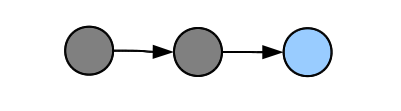
\includegraphics[width=0.3\textwidth]{partial.png}}
  \subfloat[Full]{\label{fig:full}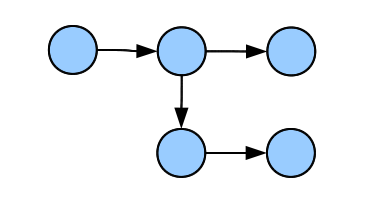
\includegraphics[width=0.3\textwidth]{fullpersistence.png}}
} \\
  \subfloat[Confluent/ Functional]{\label{fig:confluent}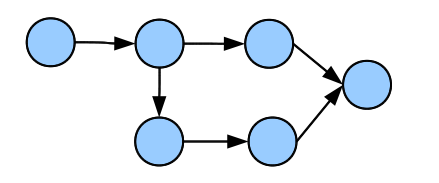
\includegraphics[width=0.3\textwidth]{confluent.png}}
 
 \caption{Version diagrams. Gray means version is read only and blue means version is read-write}
  \label{fig:version-diagrams}
\end{figure}

\section{Partial persistence}


\paragraph{Question:}
Is it possible to implement partial persistence efficiently?

\paragraph{Answer:}
Yes, assuming the pointer machine memory model and the restricting {\em in-degrees} of data nodes to be O(1). This result is due to Driscoll, Sarnak, Sleator, and Tarjan \cite{dsst}.

\paragraph{Proof idea:}
We will expand our data nodes to keep a modifications a.k.a. mods `log'. When we have modified a node enough, we create a new node to take all further updates until it also fills. 

For every node in our old data structure, the new data structure will have a collection of nodes: one current with the latest versions and potentially many old ones used only for reading the old versions. Every time we `archive' a node we will also update all (versioned) pointers to to instead refer to the latest node.

\subsection{Proof:}

We extend our data nodes to contain the following information:

\begin{enumerate}
\item a read only area for data and pointers (corresponding to those in the original structure)
\item (new) a writeable  area for back pointers. Node \(x\) has one backpointer to a node \(y\) if \(y\) has a pointer to \(x\).
This area has limited size, since we know ahead of time there are at most $p$ pointers to our node.
\item (new) a writable modifications (`mods') area for entries of the form \verb|(field, version, value)|. The size of this 
area also needs to be fixed, and it also has important consequences for write performance.
\end{enumerate}

For an illustration of the construction check figures \ref{fig:ephemeral} and \ref{fig:persistent1}

We implement read and write operations as follows:

\begin{enumerate}
\item {{\code read(var, v)}} search the mod log for the largest version \(w\) such that  \( w \leq v \). 
What if the value is in an `old' node?  then we would have gotten to it via an old version of a pointer (c.f. Figure~\ref{fig:persistent2} and Figure~\ref{binary-tree}).

\item {{\code write(var, val)}}

if \(n\) is not full, simply add to mod log.
if \(n\) has no space for more mod logs, 
\begin{itemize}
\item \(n' = \mbox{new Node()}\)
\item copy {\em latest} version of each field (data and forward pointers) to the static field section.
\item also copy back pointers to \(n'\)
\item for every node \(x\) such that \(n\) points to \(x\), redirect its back pointers to \(n'\) (using our pointers to get to them) (at most d of them).
\item for every node \(x\) such that \(x\) points to \(n\), call {\code write(x.p, n')} recursively (at most p recursive calls).

\end{itemize}
\end{enumerate}

\begin{figure}
  \centering
  \subfloat[Ephemeral linked structure. It has one data field and one pointer field]{\label{fig:ephemeral}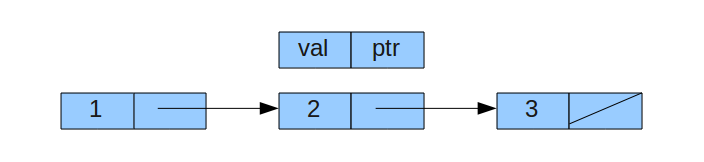
\includegraphics[scale=0.4]{3NodesDiagram1.png}}\\
  \subfloat[The structure in \ref{fig:ephemeral} partially persistent. Showing one update: {\texttt write(root.ptr.val = 20)}]{\label{fig:persistent1}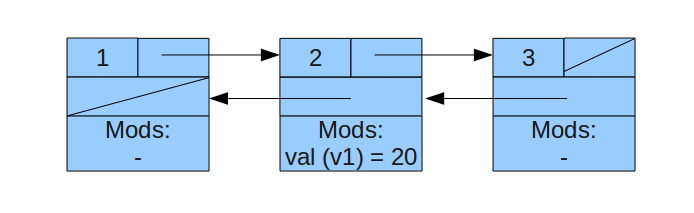
\includegraphics[scale=0.4]{3NodesDiagram2.png}}\\
  \subfloat[The structure in ~\ref{fig:persistent1} after a second update: {\ttfamily write(root.ptr.val = 200)}. Gray indicates the data node is read only]{\label{fig:persistent2}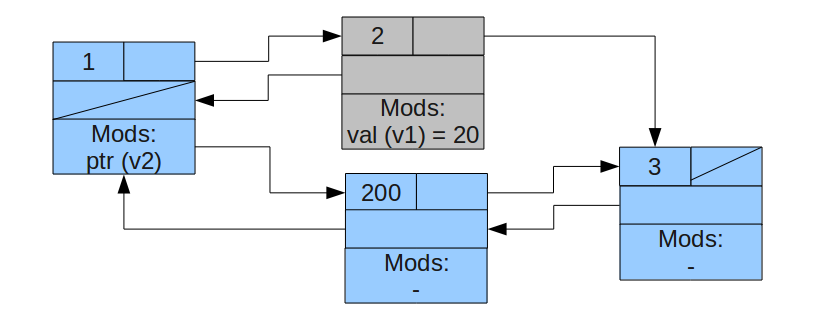
\includegraphics[scale=0.4]{3NodesDiagram3.png}}
  \caption{Constructing a partially persistent structure from an ephemeral one}
  \label{fig:partial-persistent}
\end{figure}

For some data structures such as lists or trees we often know what $p$ is ahead of time, so we can implement the algorithm for these specific structures like in figure~\ref{binary-tree}. 

\begin{figure}[h]
  \begin{center}
    \scalebox{0.6}{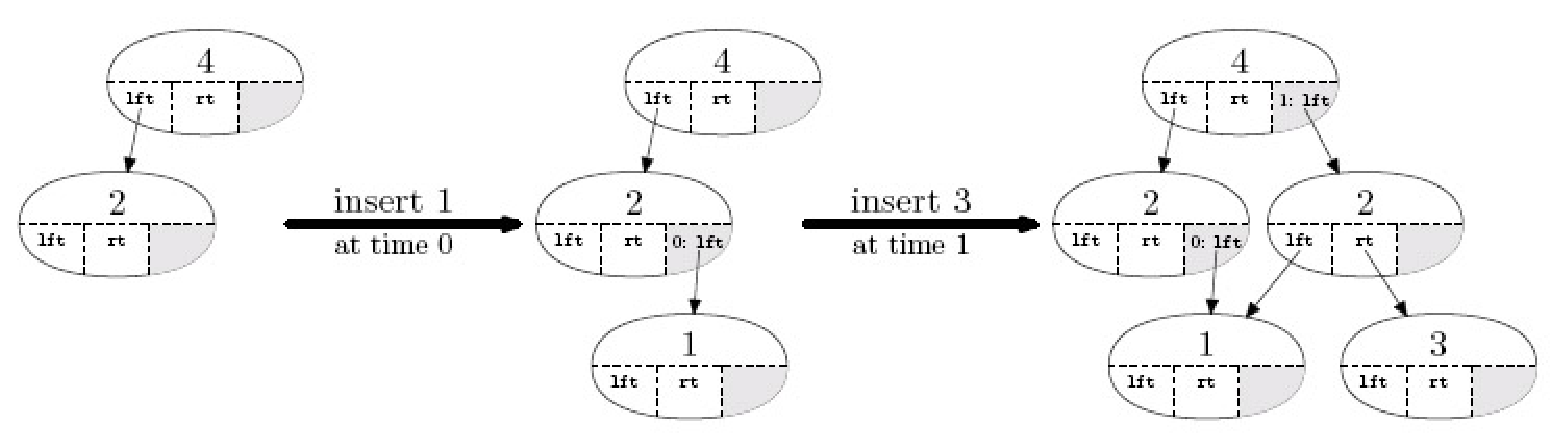
\includegraphics{ptree.pdf}}
  \end{center}
  \caption{\small Persistence of a binary tree. We need a modification box the size of the in-degree of each data structure node (just one for trees).}
  \label{binary-tree}
\end{figure}

\subsection{Analysis:}

\begin{itemize}
\item Space:

If we choose the mod log to be bounded at size \(2p\) then node has size \(d + p + 2p\) which is also \(O(1)\) because we assumed there were only \(p \leq O(1)\) pointers into any node. The reasons for choosing such a mod log size are clarified in the following cost analysis.

\item Time:
A read is cheap, it requires constant time to check through a single node's mod log and pick the required version. A write is also cheap if we have space in the mod log. If not, a write can be expensive. Let $\mbox{cost}(n)$ denote the cost of writing to node $n$. In the worst case the algorithm makes recursive calls so we get:

\[\mbox{cost}(n) = c  +  \sum_{\mbox{$x \to n$}}(\mbox{cost}(x))\]

Where $c$ represents the \(O(1)\) cost of determining latest versions to copy into the new node, copying backpointers, etc. $x \to n$ stands for $x$ points to $n$. 

Clearly the cost can be large because we could split many data nodes in the recursive steps.  However, we know when a node becomes full then next operation will likely find a more empty mod log.  For that reason amortized analysis more appropriate for this operation than worst case analysis.

Recall the potential method technique explained in \cite{clrs}: if we know a potential function $\phi$, then  \(\mbox{amortized\_cost}(n) = \mbox{cost}(n) + \Delta \phi \). 

Consider the following potential function:

\[\phi = c * \mbox{\# mod log entries in \emph{current} data nodes} \]

Since the node was full and now it is empty, the change in potential associated with our new node is $-2cp$. So now we can write a recursive expression for our amortized cost: 

\[\mbox{amortized\_cost}(n) \leq c + c - 2cp + p*\mbox{amortized\_cost}(x) \]

For some worst case node $x$. The second $c$ covers the case where we find space in our mod log, and simply add an entry to it thus increasing potential by $c$.

By unfolding the recursion once we can see at each unfolding the \(-2cp\) cancels out the extra cost from the recursion leaving only the $2c$ cost. Hence cost is \(O(1)\) amortized.   The recursion process is guaranteed to finish despite potential cycles in the graph, because splits decrease $\phi$ and $\phi$ is non-negative.

Further study by Brodal \cite{brodal} has shown actual cost to also be  \(O(1)\) in the worst case.

\end{itemize}

\section{Full persistence}
The construction for partial persistence can be expanded to implement full persistence. This result is also due to \cite{dsst}. We again assume a pointer machine with $p <  O(1)$ incoming pointers per node. 

We need to take care of a two new problems: 

1) Now we need  to represent versions in a way that lets us efficiently check which precedes which. Versions form a tree, but traversing it is \(O(\mbox{\#~of~versions})\). 

2) Now we have to support writes to any version. This affects how we handle writes: we no longer have the concept of `current' vs. `old' nodes: every node needs to support writes. 

\subsection{Version representation}

The version representation problem is solved by keeping a tree representing the version structure, as well as an efficient representation of this tree in a linearized way. 

The linearized representation of the tree in the figure~\ref{tree-traversal} is \(ba, bb, bc, ec, eb, bd, ed, ea\). You can read $ba$ as `begin node $a$' and $ea$ as `end node $a$'.  This representation losslessly encodes the tree,  and we can directly answer queries about the tree using that encoded representation. For example we know $c$ is nested within $b$, since \(bb < bc\)  and \(ec < eb\). 

\begin{figure}[h]
  \begin{center}
        \scalebox{.4}{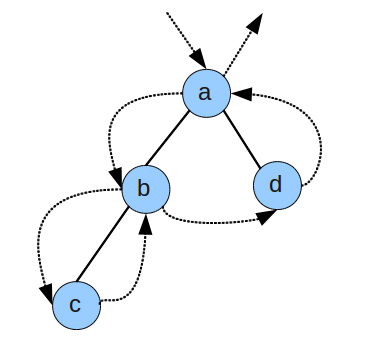
\includegraphics{TreeTraversal.png}}
  \end{center}
  \caption{\small in-order tree traversal}
  \label{tree-traversal}
\end{figure}

This linearized representation can be implemented using an `order maintenance' data structure. For now, it suffices to say an order maintenance data structure supports the following two operations, both in \(O(1)\) time.

\begin{itemize}
\item insert an item  before or after a specified element.
\item check if item $s$ precedes item $t$. 
\end{itemize}

For example, a linked list supports insertions in \(O(1)\), but tests for precedence take \(O(n)\). Similarly, a balanced BST supports both operations but in \(O(\log{n})\) time.  Deitz and Sleator show an \(O(1)\) implementation for both operations in \cite{dietz}, which will be covered in \href{http://courses.csail.mit.edu/6.851/spring12/lectures/L08.html}{lecture 8}.

To implement version tree queries such as `is version $v$ an ancestor of version $w$' we can use two comparison queries $bv < bw$ and $ew < ev$ in \(O(1)\). To implement  updates like  `add version $v$ as a child of version $w$' we can insert the two elements $bv$ and $ev$ after $bw$ and before $ew$ respectively, also in \(O(1)\). 

\subsection{Construction and algorithm:}

The nodes in our data structure will keep the same kinds of additional data per node as they did in the partially persistent case. 

For each node we store $d$ data entries and $p$ back pointers, but now allow up to $2(d+p+1)$ modifications. The amount of data $d$ is also a bound on {\em out-pointers} per node. Additionally we now also version back-pointers.

\begin{enumerate}
\item {{\code read(n.field, version)}}:
By using the order-maintenance data structure we can pick the most recent ancestor of \verb|version| from among the entries in the mod log and return that value.

\item {{\code write(n.field, value, version)}}: 
If there is space in node, just add mod entry.
else: 
\begin{itemize}
\item $m = \mbox{new Node()}$. Split the contents of node $n$'s mod log into {\em two} parts following the diagram figure~\ref{version-split}. Partitioning into subtrees rather than arbitrarily is required.

Now node $m$ has some of the mods of the internal tree in Figure~\ref{version-split}, and node $n$ retains the `older' half of the updates.

\item from the `old' mod entries in node $n$, compute the latest values of each field and write them into the data and back pointer section of node $m$.
\item recursively update all (up to)  $d + p + (d + p + 1)$ forward and backward pointers of neighbors.
\item insert new version to our version tree representation.
\end{itemize}

\end{enumerate}

\begin{figure}
  \begin{center}
        \scalebox{.4}{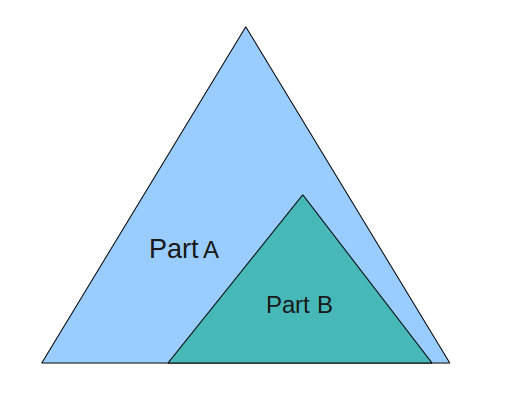
\includegraphics{VersionSplitting.png}}
  \end{center}
  \caption{\small Splitting a tree-shaped version genealogy into two subtrees}
  \label{version-split}
\end{figure}


\subsection{Analysis:}
\begin{itemize}
\item space -- 1 if we do not split or \(d + p + 2(d  + p + 1) = 3d + 3p + 2\) when we split a node, both \( O(1) \)
\item time -- \verb!read(var, version)! is implemented in a similar way to the partial case. We use our auxiliary version tree data structure to find the largest ancestor of \verb!version! from among a list of \(O(1)\) elements in \(O(1)\). 

Like with the partial case, writes are cheap when a node has space in its mods log and  more expensive when nodes are full. 
%potential function trouble: need it to change negatively, but this can only increase.
%also update partial case.

Consider \( \phi =  -c(\mbox{\# empty slots}) \), then  when we split  \( \Delta \phi = -2c(d + p + 1) \) and when we do not \(\Delta \phi = c\). Hence, \(\mbox{amortized\_cost}(n) \leq c + c - 2c(d + p + 1) + (d + p + (d + p + 1))*\mbox{amortized\_cost(x)})\) for the worst possible choice of $x$ from the neighbors.  When we unfold the recursion once,  we find the constants cancel out: \( c - 2c(d+p+1) + (2p + 2p + 1)c = 0\).
\end{itemize}

{\bf OPEN:} De-amortization of full persistence.\\
{\bf OPEN:} Is there a matching lower bound for both full and partial persistence?\\

\section{Confluent Persistence}
Confluent persistence presents new challenges. Firstly, we again need to find a new representation of versions. Our tree traversal technique is does not extend to DAGs.  Also, it is possible to have $2^u$ paths in version history after after $u$ confluent updates. For example by concatenating a string with itself repeatedly we get a version diagram like that in figure~\ref{exponential-paths}.

Deques (double ended queues allowing stack and queue operations) with concatenation can be done in constant time per operation (Kaplan, Okasaki, and Tarjan \cite{kot}). Like with a string, we can create implicitly exponential deques in polynomial time by recursively concatenating a deque with itself. 

The general transformation due to Fiat and Kaplan \cite{fiat} is as follows:

\begin{itemize}
\item \(e(v) = 1 + \log(\mbox{\# of paths from root to $v$})\). This measure is called the `effective depth' of the version DAG: if we unravel the tree via a DFS (by making a copy of each path as if they didn't overlap) and rebalanced that tree this is the best we could hope to achieve. 
\item $d(v)$ = depth of node $v$ in version DAG
\item overhead: \( \log(\mbox{\# of updates}) + \max_v(e(v))\)
\end{itemize}

This results reflects poor performance when $e(v) = 2^{u}$ where $u$ is the number of updates. This is still exponentially better than the complete copy.

\begin{figure}[h]
  \begin{center}
    \scalebox{.3}{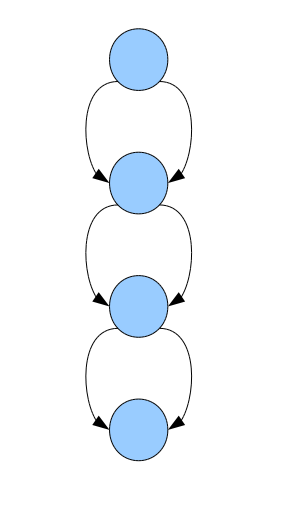
\includegraphics{exponential-paths.png}}
  \end{center}
  \caption{\small An example of $e(v)$ being linear on the number of updates.}
  \label{exponential-paths}
\end{figure}

A lower bound also by Fiat and Kaplan is \(\Omega(e(v))\) for update if queries are free. Their construction makes \(e(v)\) queries per update.

{\bf OPEN:} \( O(1) \) or even \( O(\log{(n)}) \) space overhead per operation.

Collette, Iacono and Langerman consider the special case of `disjoint operations': confluent operations performed only between versions with no shared data nodes. From there they show \( O(\log{(n)})\) overhead is possible for that case.

If we only allow disjoint operations, then each data node's version history is a tree. When evaluating  {\code read(node, field, version)} there are tree cases: when node modified at {\code version}, we simply read the new version. Where node along path between modifications, we first need to find the last modification. This problem can be solved with use of `link-cut trees' (see  \href{http://courses.csail.mit.edu/6.851/spring12/lectures/L19.html}{lecture 19}). Finally,  when {\code version} is below a leaf the problem is more complicated.  The proof makes use of techniques such as fractional cascading which will be covered in \href{http://courses.csail.mit.edu/6.851/spring12/lectures/L03.html}{lecture 3}.  The full construction is explained in \cite{collette}.

\section{Functional persistence}
Functional persistence and data structures are explored in \cite{okasaki}.  Simple examples of existing techniques include the following.

\begin{itemize}
\item {\emph{Functional balanced BSTs}} --  to persist BST's functionally, the main idea (a.k.a. `Path copying') is to duplicate the  modified node and propagate pointer changes by duplicating all ancestors. If there are no parent pointers, work top down. This technique has an overhead of \(O(\log{(n)})\) per operation, assuming the tree is balanced. Demaine, Langerman, Price show this for link-cut trees as well \cite{dlp}.

\item {\emph{Deques}} -- (double ended queues allowing stack and queue operations) with concatenation can be done in constant time per operation (Kaplan, Okasaki, and Tarjan \cite{kot}). Furthermore, Brodal, Makris and Tsichlas show in \cite{bmt} it can  be done with concatenation in constant time and update and search in $O(\log{(n)})$

\item {\emph{Tries}} -- with local navigation and subtree copy and delete. Demaine, Langerman, Price show how to persist this structure optimally in \cite{dlp}.

\end{itemize}
%% \begin{center}
%% \begin{tabular}{|l|l|l|l|}
%%   \hline
%%    & \multicolumn{2}{|c|}{finger move} & modification\\
%%   \hline
%%   method & time& space & (time = space)\\
%%   \hline
%%   path copying & $\lg{\Delta}$ & $O(1)$ & depth\\
%%   \hline
%%   1. functional & $\lg{\Delta}$ & $\lg \Delta$ & $\lg \Delta$\\
%%   \hline
%%   1. confluent & $\lg{\lg{\Delta}}$ & $\lg{\lg{\Delta}}$ & $\lg{\Delta}$\\
%%   \hline
%%   2. functional & $\lg{\Delta}$ & $O(1)$ & $\lg{n}$\\
%%   \hline
%%   2. confluent & $\lg{\lg{\Delta}}$ & $O(1)$ & $\lg{n}$\\
%%   \hline
%% \end{tabular}
%% \end{center}
%% The (1.) functional and confluent persistence data structures are cheap with local modifications. The (2.) data structures are globally balanced.

Pippenger shows at most $\log{()}$ cost separation of the functional version from the regular data structure  in \cite{pippenger}.

{\bf OPEN:} (for both functional and confluent) bigger separation? more general structure transformations? 

{\bf OPEN:} Lists with split and concatenate? General pointer machine? 

{\bf OPEN:} Array with cut and paste? Special DAGs?

\bibliography{mybib}
\bibliographystyle{alpha}

\begin{thebibliography}{77}

\bibitem{brodal}
Gerth Stølting Brodal: \emph{Partially Persistent Data Structures of Bounded Degree with Constant Update Time}. Nord. J. Comput. 3(3): 238-255 (1996)

\bibitem{dil}
Erik D. Demaine, John Iacono, Stefan Langerman: \emph{Retroactive data structures}. SODA 2004: 281-290

\bibitem{dlp}
Erik D. Demaine, Stefan Langerman, and Eric Price: \emph{Confluently Persistent Tries for Efficient Version Control}. Algorithmica (2008).

\bibitem{dietz}
Paul F. Dietz, Daniel Dominic Sleator: \emph{Two Algorithms for Maintaining Order in a List} STOC 1987: 365-372

\bibitem{dietz1}
Paul F. Dietz: \emph{Fully Persistent Arrays (Extended Array)}. WADS 1989: 67-74

\bibitem{dsst}
James R. Driscoll, Neil Sarnak, Daniel Dominic Sleator, Robert Endre Tarjan: \emph{Making Data Structures Persistent}. J. Comput. Syst. Sci. 38(1): 86-124 (1989)

\bibitem{gk}
Yoav Giora, Haim Kaplan: \emph{Optimal dynamic vertical ray shooting in rectilinear planar subdivisions} ACM Transactions on Algorithms 5(3) (2009)

\bibitem{kot}
Haim Kaplan, Chris Okasaki, Robert Endre Tarjan: \emph{Simple Confluently Persistent Catenable Lists}. SIAM J. Comput. 30(3): 965-977 (2000)

\bibitem{fiat}
Amos Fiat, Haim Kaplan: \emph{Making data structures confluently persistent}. J. Algorithms 48(1): 16-58 (2003)

\bibitem{okasaki}
Chris Okasaki: \emph{Purely Functional Data Structures}. New York: Cambridge University Press, 2003.

\bibitem{collette}
Sebastien Collette, John Iacono, and Stefan Langerman. \emph{Confluent Persistence Revisited.} In Symposium on Discrete Algorithms (SODA), pages 593-601, 2012.

\bibitem{clrs}  
T.~H. Cormen and C.~E. Leiserson and R.~L. Rivest and C.~Stein,   \emph{Introduction to Algorithms}. 3rd. Edition. The MIT Press, 2009.

\bibitem{pippenger}
Nicholas Pippenger. \emph{Pure Versus Impure Lisp}. ACM Transactions on Programming Languages and Systems, Vol. 19, No. 2. (March 1997), pp. 223-238.

\bibitem{bmt}
Gerth Stølting Brodal, Christos Makris, Kostas Tsichlas: \emph{Purely Functional Worst Case Constant Time Catenable Sorted Lists.} ESA 2006: 172-183

\end{thebibliography}

\end{document}
